\documentclass[11pt,a4paper]{article}
\usepackage{color}
\usepackage{amsmath, amsthm, amssymb, amsfonts, verbatim}
\usepackage{graphicx}
\usepackage[table,x11names]{xcolor}
\title{Assessing glymphatic transport velocities by adjoint methods}

\renewcommand{\comment}[1]{\textcolor{red}{#1}}

\author{Lars Magnus Valnes, Sebastian K. Mitusch, Geir A. Ringstad, Per Kristian Eide, Simon W. Funke, Kent-Andre Mardal }


\begin{document}
\maketitle

\begin{abstract}
\end{abstract}
\section{Introduction}

The discovery of the paravascular pathway in 2011~\cite{iliff2012paravascular} propose a novel component
crucial to the metabolism of the brain which may potientially provide an explanation for the accumulation of
waste such as amyloid beta in elderly, ultimately leading to diseases such as Alzheimer and Parkinson. 
In the rest of our body, the lymphatic system plays an important role
in the clearance of metabolic waste, but there are no lymphs within the brain. This fact is puzzling in particular because
the brain requires around 10 times more energy per volume than the result of the body. The paravascular 
pathway is proposed important to waste clearance and has therefore been named the \emph{glymphatic system}.      

The pioneering works of Sykov{\'a} and Nicholson~\cite{sykova2008diffusion} demonstrated
that diffusion was a governing transport mechanism in the brain. However, 
the clearance of CSF-tracers during sleep~\cite{xie2013sleep} in mice demonstrated transportation
much faster what could be explained by diffusion and it was proposed that arterial pulsation powered
accelrated perivascular flow combined convective interstitial flow. Several modelling attempts
have put the theory to the test~\cite{asgari2016glymphatic, smith2017glymphatic, holter2017interstitial}, 
but so far computational modeling have failed to adequately described the mechanism.   

Transportation by diffusion is in the order of XXX\comment{Lars: hente fra R. Thorne / Nicholson}. 
However, in \cite{xie2013sleep} a 60% coverage of 3kDa Texas Red Dextran of a $200 \mu m$ cube was demostrated in approximately 
20 minutes. As such, the transportation is XXX faster than what diffusion would provide. Furthermore, 
in \cite{eidevalnes} it was demonstrated that X Da Gadovist was brainwide in 8 hours after injection in the lumbar region.      

Paragraph about timescales etc. 

The purpose of this paper is to attempt to assess transportation speed in terms of an apparent diffusion coefficient 
by using adjoint methods provided by \cite{} for optimizing the coefficient with respect to data. As
such a coefficient larger than commonly reported values of diffusion would suggest that at the
timescale of minutes to hours there is indeed a glymphatic transportation which may potentially 
be responsible for metabolic waste.     

An outline of the paper is as follows. In Section 2 we descibe the medical images and their modality,  
and the mathematical methodology used for determining the apparent diffusion coefficients.  


\section{Methods}


\subsection*{Data}
The data consist of a total of 10 MRI observations, including a baseline MRI taken before tracer was injected. The observation points are distributed with 5 observations within 1-2 hours after injection, 1 observation in the timeframes 2-4 hours, 6-9 hours, 24 hours and 48 hours. 




\subsection*{Mathematical Model}
The objective function was defined as 
\begin{equation}
\min_{u,g} F = \quad \sum\limits_i\sp{n} \int\limits_{\Omega} |u(t_i) - u_{obs}(t_i)| \mathrm{d}\Omega + \frac{\alpha}{2} \int\limits_{0}\sp{T} || g ||_{L\sp{2}(\partial\Omega)} \mathrm{d}t + \frac{\beta}{2} \int\limits_{0}\sp{T} || \dot{g} ||_{L\sp{2}(\partial\Omega)}\mathrm{d}t 
\label{EQ::objf}
\end{equation}
subjugated by   
\begin{equation}
\begin{aligned}
\frac{\partial u}{\partial t} = \nabla \cdot  D_i \nabla u \qquad \text{in} \qquad \Omega \times \left\lbrace 0 , T \right)  \\
u=g(t) \qquad \text{on} \qquad \partial\Omega  \times \left\lbrace 0 , T \right) 
\end{aligned}
\label{Eq::PDE}
\end{equation}
with the domain $\Omega$ contains three sub domains, each with a different diffusion coefficient. We denote the Cerebral Spinal fluid (CSF) domain as $\Omega_1$, the grey matter as $\Omega_2$ and the white matter as $\Omega_3$.

\section*{Manufactured Solution}
The manufactured observations was obtained by forward computation of Eq.\ref{Eq::PDE} with the Dirichlet boundary condition defined as
\begin{equation}
g(t)_{\partial \Omega_1} = 0.3 +0.167t - 0.007t\sp{2} \qquad  0 \leq t \leq 24.
\end{equation}
The timestep was $dt = 0.02$, and the diffusion coefficients were selected to be 
\begin{equation}
D_{\Omega_1} = 1000 \quad , \quad D_{\Omega_2} = 4.0 \quad , \quad D_{\Omega_3} = 8.0 
\end{equation}  
The magnitude order of the diffusion coefficient are chosen so that they resemble diffusion coefficient in csf, grey and white matter. The forward simulation gave a total of 120 possible observation time points. These points 
will be denoted as $\tau$.

The mesh is patient-specific and was constructed by using the MRI of a patient diagnosed with iNPH. The software Freesurfer was used in segmentation and creating the polyhedral surfaces of the white and grey matter. Then the use of T2 weighted MRI was used to segment the csf compartment surrounding the cerebral. (BrainMesh code accessibility ? ) CGAL[?] was used to combine the polyhedral surfaces and to construed the mesh. The computational requirement for the resulting mesh was significant, therefore a submesh was also constructed, see Fig. ??. 


\section*{Implementation}
The code used the FEniCS project to sole the PDE, using backwards Euler time discretization and first order continuous Galerkin finite elements. The module dolfin adjoint [?] was used to compute the reduced functional, and the optimization used the scipy optimize library to minimize the functional using L-BFGS-B algorithm.   

The implementation used the first observation as initial conditions of Eq.\ref{Eq::PDE}, and for each timestep, the next observation was used as the Dirichlet boundary condition. The Dirichlet boundary condition was imposed on the external boundary for the domain $D_{\Omega_1}$. 



Linear interpolation of the forward problem was used to compute the difference from the observation,

The initial values of the optimization algorithm was chosen to be $1,1,1$. Furthermore, to obtain faster convergence in the optimization, the diffusion coefficients was scaled to have the same magnitude, i.e.  $D_{\Omega_1}$ was scaled, so that $D_{\Omega_1} = D\sp {s}_{\Omega_1}100$.     


The noise susceptibility was also tested by adding an uniform distribution noise term to the observations. The noise term was constructed using numpy random and multiplied with a noise amplitude. The noise amplitudes were chosen to be $ 5\%, 10\%, 50\%, 100\%$ of the maximum initial boundary conditions, so that negative concentrations are avoided.  



\section*{Non-linear relation}
The MR images are provided by Oslo University Hospital Rikshospitalet and can be seen in Fig.??. The software Freesurfer was used to segment and align each of the observations, which made it possible to estimate voxelwise intensity increase. The tracer causes the longitudinal(spin-lattice) relaxation time $T_{1}$ to shorten with the following relation
\begin{equation}
\frac{1}{T_{1}\sp{c}} = \frac{1}{T_{1}\sp{0}} + r_{1}*C .
\label{EQ::contrast}
\end{equation}
The superscripts indicating with contrast and without contrast and $r_1$ as the relaxivity constant for the MRI-contrast in a medium. The relation between intensity and the relaxation time is non-linear, and is expressed with the following equations. The signal intensity $SI$ of the sequence is given by
\begin{equation}
SI = M_{n} \sin \theta e\sp{ - TE/T_2\sp{*} },
\label{EQ::SI_T2}
\end{equation}
with  $TE$ and $\theta$ respectively denoting the echo time and the flip angle. Also $T2\sp{*}$ is transverse magnetization caused by a combination of spin-spin relaxation and magnetic field inhomogeneity. It is defined as 
\begin{equation}
\frac{1}{T_2\sp{*}} = \frac{1}{T_2} + \gamma \Delta B_{in} ,
\end{equation}
with $T2$ transverse (spin-spin) relaxation time, $\gamma$ is the gyromagnetic ratio and $\Delta B_{in}$ is the magnetic field inhomogeneity across a voxel. The expression can be simplified by neglecting the $T2$ term in the signal, since $TE <<T_2\sp{*}$ for this MRI sequence. Thus Eq. \ref{EQ::SI_T2} becomes 
\begin{equation}
SI = M_{n} \sin \theta.
\label{EQ::SI}
\end{equation}
In article [?], the term $M_n$ is defined as the magnetization for the n-echo 
\begin{equation}
M_{n} = M_{0}  \left[ (1-\beta)\frac{(1-(\alpha \beta)\sp{n-1} }{1-\alpha\beta} + (\alpha \beta)\sp{n-1}(1-\gamma) + \gamma ( \alpha \beta)\sp{n-1} \frac{M_{e}}{M_{0}}  \right]   
\end{equation}
with 
\begin{equation}
\frac{M_{e}}{M_{0}} = - \left[ \frac{ 1 -\delta + \alpha \delta (1-\beta ) \frac{1-\alpha\beta\sp{m}}{1-\alpha \beta} + \alpha\delta(\alpha\beta)\sp{m-1} - \alpha\sp{m}\rho}{1 +\rho \alpha\sp{m} } \right].
\end{equation}
Using the following definitions
\begin{equation}
\begin{aligned}
\alpha &= \cos ( \theta ) \\
\beta  &= e\sp{- \sp{T_b}/_{T_1}\sp{0} } \\
\delta &= e\sp{- \sp{T_a}/_{T_1}\sp{0} } \\
\gamma &= e\sp{- \sp{T_w}/_{T_1}\sp{0} } \\
\rho   &= e\sp{- \sp{TR}/_{T_1}\sp{0} }  \\
T_w    &= TR - T_a -T_b(m-1)       .\\
\end{aligned}
\end{equation}
Here $T_b$ is known as the echo spacing, $T_a$ is the inversion time, $T_w$ the time delay, $TR$ as the repetition time, $m$ is the number of echo spacings and $T1$ is the longitudinal(spin-lattice) relaxation time for a given medium. The $M_0$ is a calibration constant of the magnetization. The center echo denoted as $n=\sp{m}/_2$ will be the signal that we will consider when estimating MRI-contrast. Given Eq.\ref{EQ::SI} we have that relative intensity increase can be written as 
\begin{equation}
\frac{SI\sp{c}}{SI\sp{0}} = \frac{ M_{n}\sp{c} \sin (\theta)}{ M_{n}\sp{0} \sin (\theta) } ,
\end{equation}
We define that  
\begin{equation}
f(T_1) = M_{n}/M_{0} ,
\label{FIG::F}
\end{equation}
which gives the following relation 
\begin{equation}
\frac{f(T_{1}\sp{c} ) }{f(T_{1}\sp{0})}  = \frac{SI\sp{c}}{SI\sp{0}} 
\end{equation}
Thus we can express the $T_1$ change due to contrast as 
\begin{equation}
f ( T_{1}\sp{c} ) = \frac{SI\sp{c}}{SI\sp{0}} f(T_{1}\sp{0}) 
\end{equation}
and we can then estimate concentration using Eq.\ref{EQ::contrast} if we know $T_{1}\sp{0}$. The $T_{1}\sp{0}$ was obtained using MRI.


 


The convergence of L-BFGS-B algorithm can be seen in Fig.??. 
\begin{itemize}
\item describe the imaging, shortly with ref to JCI  
\item describe the abstract mathematical problem to be solved, ie. PDE constrained opt problem where we 
address coefficients and bc  
\item the details: finite element, reduced problem, BFGS,  
\end{itemize}

\begin{figure}
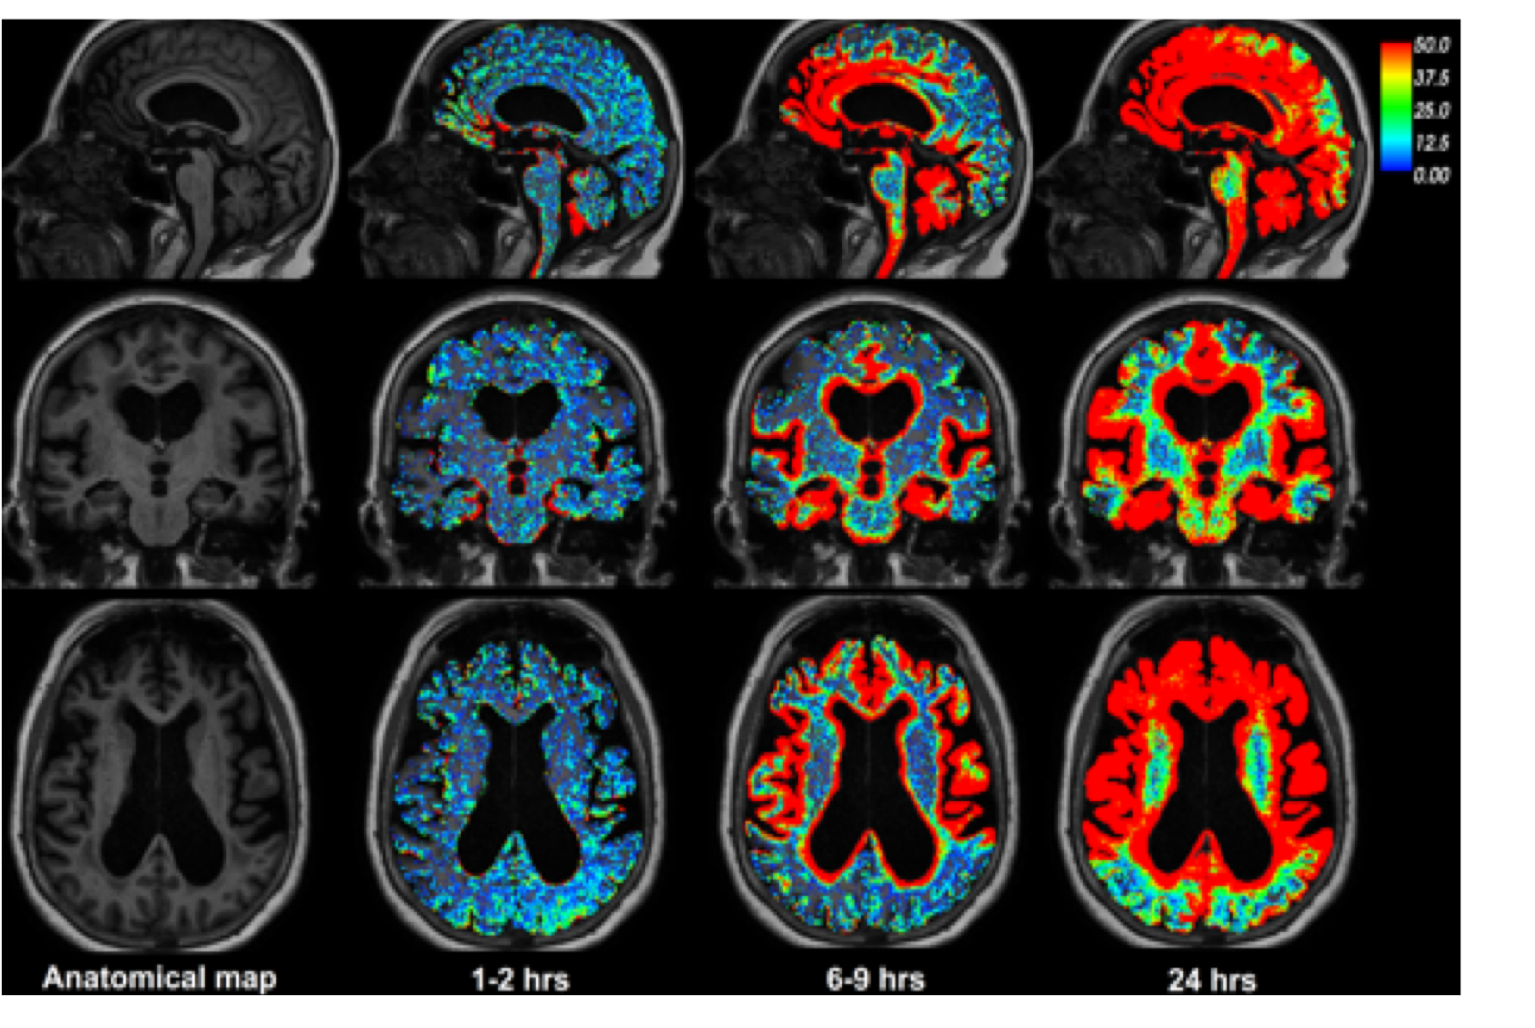
\includegraphics[width=0.95\textwidth]{GMRI.png} 
\label{fig1} 
\caption{\comment{lars, we will need some new images since I believe this is stolen from JCI}}
\end{figure}

\comment{Lars: bilde av konkret mesh  }

\begin{figure}
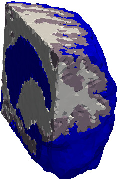
\includegraphics[width=0.3\textwidth]{mesh-eps-converted-to.pdf} 
\label{fig1} 
\caption{\comment{lars, we will need some new images since I believe this is stolen from JCI}}
\end{figure}


\section{Results}
\begin{itemize}
\item 2D experiments as have already been done (with and without noise/ with and without observations everywhere in time) 
\item 2D experiments should highlight the impact of the regularization parameter wrt number of iterations and diffusion 
coeff 
\item 3D experiments based on data generated  
\item 3D experiments based on real data (\comment{lars: we need to try testing this}) 
\end{itemize}



\begin{table}
\centering
\caption{Shows the relaxation parameters $\alpha$ and $\beta$, number of timesteps $k$ and number of observation $\tau$ with the resulting number of iterations and estimated optimal parameters for the diffusion coefficients. }
\resizebox{\textwidth}{!}{\begin{tabular}{*{8}c}
$\alpha$ & $\beta$ & k  & iter & $ D_{\Omega_1} = 1000$ & $ D_{\Omega_2} = 4.0 $ & $D_{\Omega_3} = 8.0 $ & $g$ \\
\hline
\rowcolor{red} 1.0e+00 	 & 1.0e+00 	 & 10 & 239 	 & +4.227 & +0.304 & +0.092 & +0.589 \\ 
\rowcolor{red} 1.0e+00 	 & 1.0e-01 	 & 10 & 234 	 & +4.272 & +0.305 & +0.091 & +0.596 \\ 
\rowcolor{red} 1.0e+00 	 & 1.0e-02 	 & 10 & 225 	 & +4.271 & +0.305 & +0.091 & +0.597 \\ 
\rowcolor{red} 1.0e+00 	 & 1.0e-03 	 & 10 & 235 	 & +4.600 & +0.304 & +0.090 & +0.597 \\ 
\rowcolor{red} 1.0e+00 	 & 1.0e-04 	 & 10 & 207 	 & +4.489 & +0.304 & +0.090 & +0.597 \\ 
\rowcolor{red} 1.0e+00 	 & 1.0e-05 	 & 10 & 193 	 & +4.271 & +0.305 & +0.090 & +0.597 \\ 
\rowcolor{red} 1.0e+00 	 & 1.0e-06 	 & 10 & 184 	 & +4.460 & +0.304 & +0.090 & +0.597 \\ 
 1.0e-01 	 & 1.0e+00 	 & 10 & 166 	 & +0.128 & +0.093 & +0.041 & +0.488 \\ 
 1.0e-01 	 & 1.0e-01 	 & 10 & 162 	 & +0.122 & +0.093 & +0.041 & +0.506 \\ 
 1.0e-01 	 & 1.0e-02 	 & 10 & 180 	 & +0.122 & +0.093 & +0.041 & +0.515 \\ 
 1.0e-01 	 & 1.0e-03 	 & 10 & 183 	 & +0.123 & +0.093 & +0.041 & +0.516 \\ 
 1.0e-01 	 & 1.0e-04 	 & 10 & 188 	 & +0.123 & +0.093 & +0.040 & +0.516 \\ 
 1.0e-01 	 & 1.0e-05 	 & 10 & 198 	 & +0.123 & +0.093 & +0.040 & +0.516 \\ 
 1.0e-02 	 & 1.0e+00 	 & 10 & 153 	 & +0.015 & +0.067 & +0.039 & +0.481 \\ 
 1.0e-02 	 & 1.0e-01 	 & 10 & 166 	 & +0.005 & +0.065 & +0.039 & +0.483 \\ 
 1.0e-02 	 & 1.0e-02 	 & 10 & 222 	 & +0.005 & +0.065 & +0.039 & +0.501 \\ 
 1.0e-02 	 & 1.0e-03 	 & 10 & 227 	 & +0.005 & +0.065 & +0.039 & +0.510 \\ 
 1.0e-02 	 & 1.0e-04 	 & 10 & 163 	 & +0.006 & +0.065 & +0.039 & +0.509 \\ 
 1.0e-02 	 & 1.0e-05 	 & 10 & 188 	 & +0.005 & +0.065 & +0.039 & +0.510 \\ 
 1.0e-03 	 & 1.0e+00 	 & 10 & 168 	 & +0.005 & +0.064 & +0.039 & +0.481 \\ 
 1.0e-03 	 & 1.0e-01 	 & 10 & 230 	 & -0.005 & +0.063 & +0.039 & +0.481 \\ 
 1.0e-03 	 & 1.0e-02 	 & 10 & 89 	 & -0.007 & +0.063 & +0.039 & +0.488 \\ 
 1.0e-03 	 & 1.0e-03 	 & 10 & 77 	 & -0.005 & +0.062 & +0.039 & +0.488 \\ 
 1.0e-03 	 & 1.0e-04 	 & 10 & 107 	 & -0.006 & +0.062 & +0.039 & +0.489 \\ 
 1.0e-03 	 & 1.0e-05 	 & 10 & 140 	 & -0.006 & +0.062 & +0.039 & +0.490 \\ 
 1.0e-04 	 & 1.0e+00 	 & 10 & 179 	 & +0.003 & +0.064 & +0.039 & +0.481 \\ 
 1.0e-04 	 & 1.0e-01 	 & 10 & 215 	 & -0.005 & +0.062 & +0.039 & +0.481 \\ 
 1.0e-04 	 & 1.0e-02 	 & 10 & 190 	 & -0.007 & +0.062 & +0.039 & +0.482 \\ 
 1.0e-04 	 & 1.0e-03 	 & 10 & 124 	 & -0.008 & +0.062 & +0.039 & +0.488 \\ 
 1.0e-04 	 & 1.0e-04 	 & 10 & 106 	 & -0.007 & +0.062 & +0.039 & +0.488 \\ 
 1.0e-04 	 & 1.0e-05 	 & 10 & 97 	 & -0.008 & +0.062 & +0.039 & +0.488 \\ 
 1.0e-05 	 & 1.0e+00 	 & 10 & 193 	 & +0.003 & +0.064 & +0.039 & +0.481 \\ 
 1.0e-05 	 & 1.0e-01 	 & 10 & 174 	 & -0.007 & +0.062 & +0.039 & +0.481 \\ 
 1.0e-05 	 & 1.0e-02 	 & 10 & 180 	 & -0.008 & +0.062 & +0.039 & +0.482 \\ 
 1.0e-05 	 & 1.0e-03 	 & 10 & 70 	 & -0.007 & +0.062 & +0.039 & +0.488 \\ 
 1.0e-05 	 & 1.0e-04 	 & 10 & 77 	 & -0.007 & +0.062 & +0.039 & +0.488 \\ 
 1.0e-05 	 & 1.0e-05 	 & 10 & 100 	 & -0.008 & +0.062 & +0.039 & +0.488 \\ 
 1.0e-06 	 & 1.0e+00 	 & 10 & 209 	 & +0.004 & +0.064 & +0.039 & +0.482 \\ 
 1.0e-06 	 & 1.0e-01 	 & 10 & 187 	 & -0.006 & +0.062 & +0.039 & +0.481 \\ 
 1.0e-06 	 & 1.0e-02 	 & 10 & 205 	 & -0.008 & +0.062 & +0.039 & +0.482 \\ 
 1.0e-06 	 & 1.0e-03 	 & 10 & 79 	 & -0.006 & +0.062 & +0.039 & +0.488 \\ 
 1.0e-06 	 & 1.0e-04 	 & 10 & 107 	 & -0.007 & +0.062 & +0.039 & +0.488 \\ 
 1.0e-06 	 & 1.0e-05 	 & 10 & 110 	 & -0.007 & +0.062 & +0.039 & +0.488 \\ 
\end{tabular}}
\label{Tab::1}
\end{table} 




\begin{table}
\centering
\caption{Shows the relaxation parameters $\alpha$ and $\beta$, number of timesteps $k$ and number of observation $\tau$ with the resulting number of iterations and estimated optimal parameters for the diffusion coefficients. }
\resizebox{\textwidth}{!}{\begin{tabular}{*{8}c}
$\alpha$ & $\beta$ & k  & iter & $ D_{\Omega_1} = 1000$ & $ D_{\Omega_2} = 4.0 $ & $D_{\Omega_3} = 8.0 $ & $g$ \\
\hline
 1.0e-01 	 & 1.0e+00 	 & 20 & 221 	 & +0.155 & +0.056 & +0.020 & +0.464 \\ 
 1.0e-01 	 & 1.0e-01 	 & 20 & 218 	 & +0.422 & +0.185 & +0.029 & +0.485 \\ 
 1.0e-01 	 & 1.0e-02 	 & 20 & 332 	 & +0.925 & +0.484 & +0.047 & +0.569 \\ 
 1.0e-01 	 & 1.0e-03 	 & 20 & 327 	 & +1.140 & +0.629 & +0.057 & +0.608 \\ 
 1.0e-01 	 & 1.0e-04 	 & 20 & 320 	 & +1.175 & +0.652 & +0.059 & +0.615 \\ 
 1.0e-01 	 & 1.0e-05 	 & 20 & 308 	 & +1.173 & +0.654 & +0.059 & +0.615 \\ 
 1.0e-02 	 & 1.0e+00 	 & 20 & 251 	 & +0.008 & +0.009 & +0.014 & +0.460 \\ 
 1.0e-02 	 & 1.0e-01 	 & 20 & 214 	 & +0.062 & +0.029 & +0.009 & +0.457 \\ 
 1.0e-02 	 & 1.0e-02 	 & 20 & 331 	 & +0.155 & +0.080 & +0.003 & +0.475 \\ 
 1.0e-02 	 & 1.0e-03 	 & 20 & 537 	 & +0.209 & +0.113 & -0.000 & +0.537 \\ 
 1.0e-02 	 & 1.0e-04 	 & 20 & 488 	 & +0.222 & +0.122 & -0.001 & +0.561 \\ 
 1.0e-02 	 & 1.0e-05 	 & 20 & 512 	 & +0.223 & +0.121 & -0.001 & +0.567 \\ 
 1.0e-03 	 & 1.0e+00 	 & 20 & 256 	 & -0.006 & +0.004 & +0.013 & +0.461 \\ 
 1.0e-03 	 & 1.0e-01 	 & 20 & 258 	 & +0.032 & +0.012 & +0.008 & +0.459 \\ 
 1.0e-03 	 & 1.0e-02 	 & 20 & 287 	 & +0.077 & +0.029 & +0.005 & +0.458 \\ 
 1.0e-03 	 & 1.0e-03 	 & 20 & 331 	 & +0.107 & +0.044 & +0.003 & +0.471 \\ 
 1.0e-03 	 & 1.0e-04 	 & 20 & 576 	 & +0.095 & +0.041 & +0.004 & +0.520 \\ 
 1.0e-03 	 & 1.0e-05 	 & 20 & 507 	 & +0.089 & +0.044 & +0.004 & +0.530 \\ 
 1.0e-04 	 & 1.0e+00 	 & 20 & 187 	 & -0.007 & +0.004 & +0.013 & +0.461 \\ 
 1.0e-04 	 & 1.0e-01 	 & 20 & 315 	 & +0.028 & +0.010 & +0.008 & +0.459 \\ 
 1.0e-04 	 & 1.0e-02 	 & 20 & 396 	 & +0.067 & +0.023 & +0.005 & +0.459 \\ 
 1.0e-04 	 & 1.0e-03 	 & 20 & 242 	 & +0.103 & +0.038 & +0.003 & +0.463 \\ 
 1.0e-04 	 & 1.0e-04 	 & 20 & 207 	 & +0.100 & +0.035 & +0.003 & +0.466 \\ 
 1.0e-04 	 & 1.0e-05 	 & 20 & 457 	 & +0.080 & +0.035 & +0.003 & +0.483 \\ 
 1.0e-05 	 & 1.0e+00 	 & 20 & 215 	 & -0.006 & +0.004 & +0.013 & +0.461 \\ 
 1.0e-05 	 & 1.0e-01 	 & 20 & 244 	 & +0.028 & +0.010 & +0.008 & +0.459 \\ 
 1.0e-05 	 & 1.0e-02 	 & 20 & 399 	 & +0.070 & +0.024 & +0.005 & +0.460 \\ 
 1.0e-05 	 & 1.0e-03 	 & 20 & 267 	 & +0.108 & +0.040 & +0.003 & +0.463 \\ 
 1.0e-05 	 & 1.0e-04 	 & 20 & 361 	 & +0.089 & +0.034 & +0.003 & +0.473 \\ 
 1.0e-05 	 & 1.0e-05 	 & 20 & 298 	 & +0.101 & +0.036 & +0.003 & +0.473 \\ 
 1.0e-06 	 & 1.0e+00 	 & 20 & 240 	 & -0.007 & +0.004 & +0.013 & +0.461 \\ 
 1.0e-06 	 & 1.0e-01 	 & 20 & 269 	 & +0.027 & +0.009 & +0.008 & +0.459 \\ 
 1.0e-06 	 & 1.0e-02 	 & 20 & 314 	 & +0.070 & +0.025 & +0.005 & +0.459 \\ 
 1.0e-06 	 & 1.0e-03 	 & 20 & 214 	 & +0.102 & +0.038 & +0.002 & +0.462 \\ 
 1.0e-06 	 & 1.0e-04 	 & 20 & 437 	 & +0.079 & +0.032 & +0.004 & +0.475 \\ 
 1.0e-06 	 & 1.0e-05 	 & 20 & 353 	 & +0.088 & +0.033 & +0.005 & +0.478 \\ 
\end{tabular}}
\label{Tab::1}
\end{table} 




\begin{table}
\centering
\caption{Shows the relaxation parameters $\alpha$ and $\beta$, number of timesteps $k$ and number of observation $\tau$ with the resulting number of iterations and estimated optimal parameters for the diffusion coefficients. Noise 0.015 amp }
\resizebox{\textwidth}{!}{\begin{tabular}{*{8}c}
$\alpha$ & $\beta$ & k  & iter & $ D_{\Omega_1} $ & $ D_{\Omega_2} $ & $D_{\Omega_3} $ & $g$ \\
\hline
 1.0e+00 	 & 1.0e+00 	 & 10 & 205 	 & +4.270 & +0.303 & +0.091 & +0.589 \\ 
 1.0e+00 	 & 1.0e-01 	 & 10 & 190 	 & +4.270 & +0.306 & +0.091 & +0.596 \\ 
 1.0e+00 	 & 1.0e-02 	 & 10 & 244 	 & +4.523 & +0.304 & +0.091 & +0.597 \\ 
 1.0e+00 	 & 1.0e-03 	 & 10 & 204 	 & +4.275 & +0.306 & +0.091 & +0.597 \\ 
 1.0e+00 	 & 1.0e-04 	 & 10 & 205 	 & +4.272 & +0.306 & +0.090 & +0.597 \\ 
 1.0e+00 	 & 1.0e-05 	 & 10 & 185 	 & +4.272 & +0.305 & +0.090 & +0.597 \\ 
 1.0e+00 	 & 1.0e-06 	 & 10 & 223 	 & +4.538 & +0.303 & +0.091 & +0.597 \\ 
 1.0e-01 	 & 1.0e+00 	 & 10 & 179 	 & +0.125 & +0.095 & +0.040 & +0.488 \\ 
 1.0e-01 	 & 1.0e-01 	 & 10 & 141 	 & +0.123 & +0.093 & +0.040 & +0.506 \\ 
 1.0e-01 	 & 1.0e-02 	 & 10 & 201 	 & +0.124 & +0.093 & +0.040 & +0.515 \\ 
 1.0e-01 	 & 1.0e-03 	 & 10 & 207 	 & +0.126 & +0.093 & +0.041 & +0.516 \\ 
 1.0e-01 	 & 1.0e-04 	 & 10 & 162 	 & +0.125 & +0.093 & +0.040 & +0.516 \\ 
 1.0e-01 	 & 1.0e-05 	 & 10 & 209 	 & +0.121 & +0.093 & +0.041 & +0.516 \\ 
 1.0e-01 	 & 1.0e-06 	 & 10 & 147 	 & +0.123 & +0.093 & +0.041 & +0.516 \\ 
 1.0e-02 	 & 1.0e+00 	 & 10 & 221 	 & +0.017 & +0.067 & +0.039 & +0.481 \\ 
 1.0e-02 	 & 1.0e-01 	 & 10 & 138 	 & +0.005 & +0.065 & +0.040 & +0.483 \\ 
 1.0e-02 	 & 1.0e-02 	 & 10 & 174 	 & +0.006 & +0.065 & +0.040 & +0.500 \\ 
 1.0e-02 	 & 1.0e-03 	 & 10 & 227 	 & +0.007 & +0.066 & +0.039 & +0.510 \\ 
 1.0e-02 	 & 1.0e-04 	 & 10 & 164 	 & +0.004 & +0.065 & +0.040 & +0.509 \\ 
 1.0e-02 	 & 1.0e-05 	 & 10 & 223 	 & +0.006 & +0.065 & +0.040 & +0.512 \\ 
 1.0e-02 	 & 1.0e-06 	 & 10 & 179 	 & +0.007 & +0.065 & +0.040 & +0.510 \\ 
 1.0e-03 	 & 1.0e+00 	 & 10 & 178 	 & +0.005 & +0.064 & +0.039 & +0.481 \\ 
 1.0e-03 	 & 1.0e-01 	 & 10 & 182 	 & -0.007 & +0.062 & +0.040 & +0.481 \\ 
 1.0e-03 	 & 1.0e-02 	 & 10 & 94 	 & -0.006 & +0.062 & +0.038 & +0.487 \\ 
 1.0e-03 	 & 1.0e-03 	 & 10 & 108 	 & -0.005 & +0.063 & +0.039 & +0.489 \\ 
 1.0e-03 	 & 1.0e-04 	 & 10 & 136 	 & -0.008 & +0.062 & +0.040 & +0.490 \\ 
 1.0e-03 	 & 1.0e-05 	 & 10 & 93 	 & -0.006 & +0.063 & +0.040 & +0.489 \\ 
 1.0e-03 	 & 1.0e-06 	 & 10 & 81 	 & -0.006 & +0.062 & +0.040 & +0.489 \\ 
 1.0e-04 	 & 1.0e+00 	 & 10 & 166 	 & +0.007 & +0.064 & +0.039 & +0.482 \\ 
 1.0e-04 	 & 1.0e-01 	 & 10 & 273 	 & -0.007 & +0.062 & +0.040 & +0.481 \\ 
 1.0e-04 	 & 1.0e-02 	 & 10 & 103 	 & -0.004 & +0.062 & +0.040 & +0.487 \\ 
 1.0e-04 	 & 1.0e-03 	 & 10 & 147 	 & -0.008 & +0.062 & +0.039 & +0.488 \\ 
 1.0e-04 	 & 1.0e-04 	 & 10 & 103 	 & -0.007 & +0.062 & +0.039 & +0.488 \\ 
 1.0e-04 	 & 1.0e-05 	 & 10 & 136 	 & -0.007 & +0.063 & +0.039 & +0.488 \\ 
 1.0e-04 	 & 1.0e-06 	 & 10 & 103 	 & -0.010 & +0.062 & +0.040 & +0.488 \\ 
 1.0e-05 	 & 1.0e+00 	 & 10 & 230 	 & +0.001 & +0.064 & +0.038 & +0.482 \\ 
 1.0e-05 	 & 1.0e-01 	 & 10 & 237 	 & -0.009 & +0.062 & +0.040 & +0.481 \\ 
 1.0e-05 	 & 1.0e-02 	 & 10 & 172 	 & -0.008 & +0.062 & +0.039 & +0.482 \\ 
 1.0e-05 	 & 1.0e-03 	 & 10 & 116 	 & -0.009 & +0.063 & +0.039 & +0.488 \\ 
 1.0e-05 	 & 1.0e-04 	 & 10 & 124 	 & -0.007 & +0.062 & +0.040 & +0.488 \\ 
 1.0e-05 	 & 1.0e-05 	 & 10 & 97 	 & -0.007 & +0.063 & +0.038 & +0.488 \\ 
 1.0e-05 	 & 1.0e-06 	 & 10 & 129 	 & -0.007 & +0.062 & +0.039 & +0.488 \\ 
 1.0e-06 	 & 1.0e+00 	 & 10 & 199 	 & +0.002 & +0.063 & +0.039 & +0.482 \\ 
 1.0e-06 	 & 1.0e-01 	 & 10 & 245 	 & -0.005 & +0.063 & +0.039 & +0.481 \\ 
 1.0e-06 	 & 1.0e-02 	 & 10 & 206 	 & -0.003 & +0.062 & +0.039 & +0.482 \\ 
 1.0e-06 	 & 1.0e-03 	 & 10 & 159 	 & -0.007 & +0.062 & +0.040 & +0.488 \\ 
 1.0e-06 	 & 1.0e-04 	 & 10 & 124 	 & -0.011 & +0.062 & +0.040 & +0.488 \\ 
 1.0e-06 	 & 1.0e-05 	 & 10 & 93 	 & -0.007 & +0.061 & +0.039 & +0.488 \\ 
 1.0e-06 	 & 1.0e-06 	 & 10 & 115 	 & -0.009 & +0.062 & +0.039 & +0.488 \\ 
\end{tabular}}
\label{Tab::1}
\end{table} 

\begin{table}
\centering
\caption{Shows the relaxation parameters $\alpha$ and $\beta$, number of timesteps $k$ and number of observation $\tau$ with the resulting number of iterations and estimated optimal parameters for the diffusion coefficients. Noise 0.15 amp }
\resizebox{\textwidth}{!}{\begin{tabular}{*{8}c}
$\alpha$ & $\beta$ & k  & iter & $ D_{\Omega_1} $ & $ D_{\Omega_2} $ & $D_{\Omega_3} $ & $g$ \\
\hline
 1.0e+00 	 & 1.0e+00 	 & 10 & 215 	 & +4.279 & +0.304 & +0.089 & +0.592 \\ 
 1.0e+00 	 & 1.0e-01 	 & 10 & 174 	 & +3.667 & +0.319 & +0.092 & +0.599 \\ 
 1.0e+00 	 & 1.0e-02 	 & 10 & 168 	 & +3.722 & +0.311 & +0.087 & +0.600 \\ 
 1.0e+00 	 & 1.0e-03 	 & 10 & 197 	 & +4.219 & +0.305 & +0.092 & +0.601 \\ 
 1.0e+00 	 & 1.0e-04 	 & 10 & 200 	 & +4.302 & +0.295 & +0.095 & +0.601 \\ 
 1.0e+00 	 & 1.0e-05 	 & 10 & 190 	 & +4.281 & +0.307 & +0.090 & +0.601 \\ 
 1.0e+00 	 & 1.0e-06 	 & 10 & 211 	 & +4.310 & +0.301 & +0.085 & +0.600 \\ 
 1.0e-01 	 & 1.0e+00 	 & 10 & 126 	 & +0.129 & +0.092 & +0.039 & +0.493 \\ 
 1.0e-01 	 & 1.0e-01 	 & 10 & 205 	 & +0.134 & +0.091 & +0.047 & +0.512 \\ 
 1.0e-01 	 & 1.0e-02 	 & 10 & 232 	 & +0.150 & +0.093 & +0.042 & +0.521 \\ 
 1.0e-01 	 & 1.0e-03 	 & 10 & 219 	 & +0.155 & +0.085 & +0.040 & +0.524 \\ 
 1.0e-01 	 & 1.0e-04 	 & 10 & 181 	 & +0.153 & +0.091 & +0.040 & +0.523 \\ 
 1.0e-01 	 & 1.0e-05 	 & 10 & 176 	 & +0.111 & +0.098 & +0.037 & +0.523 \\ 
 1.0e-01 	 & 1.0e-06 	 & 10 & 151 	 & +0.155 & +0.092 & +0.043 & +0.523 \\ 
 1.0e-02 	 & 1.0e+00 	 & 10 & 214 	 & +0.014 & +0.066 & +0.038 & +0.486 \\ 
 1.0e-02 	 & 1.0e-01 	 & 10 & 139 	 & +0.007 & +0.072 & +0.034 & +0.490 \\ 
 1.0e-02 	 & 1.0e-02 	 & 10 & 235 	 & +0.032 & +0.076 & +0.041 & +0.512 \\ 
 1.0e-02 	 & 1.0e-03 	 & 10 & 282 	 & +0.002 & +0.067 & +0.041 & +0.519 \\ 
 1.0e-02 	 & 1.0e-04 	 & 10 & 353 	 & +0.002 & +0.060 & +0.043 & +0.523 \\ 
 1.0e-02 	 & 1.0e-05 	 & 10 & 324 	 & +0.043 & +0.067 & +0.042 & +0.521 \\ 
 1.0e-02 	 & 1.0e-06 	 & 10 & 261 	 & +0.028 & +0.069 & +0.037 & +0.525 \\ 
 1.0e-03 	 & 1.0e+00 	 & 10 & 222 	 & +0.013 & +0.061 & +0.035 & +0.488 \\ 
 1.0e-03 	 & 1.0e-01 	 & 10 & 227 	 & +0.002 & +0.069 & +0.041 & +0.489 \\ 
 1.0e-03 	 & 1.0e-02 	 & 10 & 341 	 & -0.015 & +0.066 & +0.038 & +0.496 \\ 
 1.0e-03 	 & 1.0e-03 	 & 10 & 309 	 & -0.018 & +0.067 & +0.033 & +0.516 \\ 
 1.0e-03 	 & 1.0e-04 	 & 10 & 406 	 & -0.034 & +0.057 & +0.049 & +0.545 \\ 
 1.0e-03 	 & 1.0e-05 	 & 10 & 400 	 & +0.011 & +0.057 & +0.042 & +0.545 \\ 
 1.0e-03 	 & 1.0e-06 	 & 10 & 349 	 & -0.004 & +0.071 & +0.042 & +0.539 \\ 
 1.0e-04 	 & 1.0e+00 	 & 10 & 186 	 & -0.031 & +0.069 & +0.039 & +0.487 \\ 
 1.0e-04 	 & 1.0e-01 	 & 10 & 230 	 & -0.004 & +0.067 & +0.030 & +0.489 \\ 
 1.0e-04 	 & 1.0e-02 	 & 10 & 264 	 & -0.032 & +0.057 & +0.044 & +0.493 \\ 
 1.0e-04 	 & 1.0e-03 	 & 10 & 302 	 & -0.026 & +0.059 & +0.039 & +0.511 \\ 
 1.0e-04 	 & 1.0e-04 	 & 10 & 417 	 & -0.020 & +0.058 & +0.040 & +0.577 \\ 
 1.0e-04 	 & 1.0e-05 	 & 10 & 598 	 & +0.004 & +0.063 & +0.041 & +0.703 \\ 
 1.0e-04 	 & 1.0e-06 	 & 10 & 554 	 & +0.011 & +0.059 & +0.038 & +0.647 \\ 
 1.0e-05 	 & 1.0e+00 	 & 10 & 232 	 & +0.019 & +0.060 & +0.039 & +0.487 \\ 
 1.0e-05 	 & 1.0e-01 	 & 10 & 216 	 & +0.011 & +0.066 & +0.040 & +0.489 \\ 
 1.0e-05 	 & 1.0e-02 	 & 10 & 340 	 & -0.044 & +0.068 & +0.042 & +0.493 \\ 
 1.0e-05 	 & 1.0e-03 	 & 10 & 369 	 & +0.000 & +0.063 & +0.034 & +0.518 \\ 
 1.0e-05 	 & 1.0e-04 	 & 10 & 561 	 & +0.005 & +0.060 & +0.031 & +0.652 \\ 
\rowcolor{red} 1.0e-05 	 & 1.0e-05 	 & 10 & 1001 	 & -0.002 & +0.066 & +0.037 & +1.226 \\ 
\rowcolor{red} 1.0e-05 	 & 1.0e-06 	 & 10 & 856 	 & -0.001 & +0.065 & +0.040 & +1.025 \\ 
 1.0e-06 	 & 1.0e+00 	 & 10 & 146 	 & +0.046 & +0.061 & +0.032 & +0.488 \\ 
 1.0e-06 	 & 1.0e-01 	 & 10 & 287 	 & -0.008 & +0.063 & +0.040 & +0.488 \\ 
 1.0e-06 	 & 1.0e-02 	 & 10 & 295 	 & +0.025 & +0.068 & +0.039 & +0.493 \\ 
 1.0e-06 	 & 1.0e-03 	 & 10 & 252 	 & +0.032 & +0.061 & +0.041 & +0.510 \\ 
 1.0e-06 	 & 1.0e-04 	 & 10 & 520 	 & +0.021 & +0.061 & +0.042 & +0.620 \\ 
\rowcolor{red} 1.0e-06 	 & 1.0e-05 	 & 10 & 1001 	 & -0.013 & +0.063 & +0.041 & +1.170 \\ 
 \rowcolor{red}1.0e-06 	 & 1.0e-06 	 & 10 & 821 	 & -0.008 & +0.066 & +0.033 & +1.079 \\ 
\end{tabular}}
\label{Tab::1}
\end{table} 
%\begin{table}
%\centering
%\caption{ $\tau = [1.0, 1.2, 1.4, 2.8, 4.6, 9.6, 14.4, 18.6, 22.2, 24.0] $}
%\resizebox{\textwidth}{!}{\begin{tabular}{*{7}c}
%$\alpha$ & $\beta$ & k & iter & $ D_{\Omega_1} = 1000$ & $ D_{\Omega_2} = 4.0 $ & $D_{\Omega_3} = 8.0 $ \\
%\hline
%
%\label{Tab::1}
%\end{table} 
%\section{Discussion}
%
%
%\begin{table}
%\centering
%\caption{ $\tau =[1.2, 1.4, 1.8, 2.4, 3.6, 5.4, 7.6, 17.2, 18.6, 20.4, 22.4, 24.0] $}
%\resizebox{\textwidth}{!}{\begin{tabular}{*{7}c}
%$\alpha$ & $\beta$ & k & iter & $ D_{\Omega_1} = 1000$ & $ D_{\Omega_2} = 4.0 $ & $D_{\Omega_3} = 8.0 $ \\
%\hline
%
%\end{tabular}}
%\label{Tab::1}
%\end{table} 
\section{Discussion}


 \begin{table}
\centering
\caption{ $\tau = [2.4, 4.8, 7.2, 9.6, 12.0, 14.4, 16.8, 19.2, 21.6, 24.0] $}
\resizebox{\textwidth}{!}{\begin{tabular}{*{8}c}
$\alpha$ & $\beta$ & k & iter & $ D_{\Omega_1} = 1000$ & $ D_{\Omega_2} = 4.0 $ & $D_{\Omega_3} = 8.0 $ & $g$ \\
\hline
 1.0e-04 	 & 1.0e+00 	 & 40 & 234 	 & -0.017 & -0.019 & +0.005 & +0.459 \\ 
 1.0e-04 	 & 1.0e-01 	 & 40 & 415 	 & +0.001 & -0.007 & +0.004 & +0.457 \\ 
 1.0e-04 	 & 1.0e-02 	 & 40 & 370 	 & +0.006 & +0.004 & +0.002 & +0.455 \\ 
 1.0e-05 	 & 1.0e+00 	 & 40 & 296 	 & -0.017 & -0.019 & +0.005 & +0.459 \\ 
 1.0e-05 	 & 1.0e-01 	 & 40 & 343 	 & +0.001 & -0.007 & +0.004 & +0.457 \\ 
 1.0e-05 	 & 1.0e-02 	 & 40 & 348 	 & +0.006 & +0.005 & +0.003 & +0.454 \\ 
 1.0e-06 	 & 1.0e+00 	 & 40 & 311 	 & -0.019 & -0.019 & +0.005 & +0.459 \\ 
 1.0e-06 	 & 1.0e-01 	 & 40 & 429 	 & -0.000 & -0.007 & +0.004 & +0.457 \\ 
 1.0e-06 	 & 1.0e-02 	 & 40 & 454 	 & +0.002 & +0.001 & +0.002 & +0.456 \\ 
 
\end{tabular}}
\label{Tab::Incoherence}
\end{table} 
\section{Discussion}


In Tab. ?? we observe that the optimal relaxation parameters are found for $\alpha := \lbrace 1.e-4 1.e-5 1.e-6 \rbrace$ and $\beta := \lbrace 1.0 0.1 0.01 \rbrace$. This will be the region of interest for the relaxation parameters.

The dependency on number of timesteps can be seen in Fig.??.






\bibliographystyle{amsplain}
\bibliography{references}


\end{document}


